\documentclass[a4paper, 10pt]{ctexart} %中文支持
\usepackage{float}              %防止浮动元素浮动
\usepackage{rotating}           %旋转图片
\usepackage{hyperref}           %生成可跳转的书签
\usepackage{amsfonts}           %对某一些字体之支持
\usepackage{amsmath}          %数学公式
\usepackage{amsthm}             %定义, 定理, 证明, 例子环境的支持
%使用方法:
%\newtheorem{environment name}{caption}
%比如 \newtheorem{example}{这是例子}
%效果 \begin{example} xxx \end{example} -> 这是例子 1 xxx
%proof就不需要了
\usepackage{graphicx}           %插入图片
\usepackage[left=1.5in,right=1.5in,top=1in,bottom=1in]{geometry}   %用来排版的
\usepackage[]{color}            %给部分文本上色的
\usepackage{algorithm}          %写伪代码的
\usepackage{algorithmic}        %同上
\usepackage{minted}             %书写代码
\usepackage{amssymb}            %用来加入一些数学符号, 比如说 $\varnothing$
\usepackage{fontspec}           %不知道用来干嘛的
\usepackage{titlesec}           %用来调整section等的大小和字体
\pagestyle{plain}
\titleformat*{\section}{\huge\bfseries}
\titleformat*{\subsection}{\Large\bfseries}
\titleformat*{\subsubsection}{\large\bfseries}
% 日, content里的不还是没变? 难堪的一笔

\setmonofont{Ubuntu Mono}       %?
\usemintedstyle{custommanni}    %设置minted插入代码的风格

\newtheorem{theorem}{定理}
\newtheorem{example}{Example}
\newtheorem{definition}{定义}
\newtheorem{lemma}{引理}
\newtheorem{proposition}{命题}
\title{single-source shortest paths}
\begin{document}
\begin{titlepage}
    \maketitle
\end{titlepage}
\tableofcontents


\section{intro and prequisition}
\subsection{Notation}

我们研究最短路径的话, 我们必然会面对图的各种参数, 因为我们当然是在有权图上面寻找最短路径的, 如果说是那种将路径长度定义为路径所经过的节点个数的话, 正如22所讲的那样的话, 
这种就不在我们这次的研究范围内了. 于是我们给定的是 {\bf 有权, 有向图}. 

\begin{definition}
    A graph is abbreviated as $G  = \left(V, E\right)$ , 这是我们已经熟知的. 
\end{definition}

\begin{definition}
一个path记为 $p$ , 可以写为 $\left< v_{0}, v_{1}, \cdots , v_{n}\right>$ , 为了突出其终点和起点, 一个path可以记为
$$p: u \leadsto v$$
\end{definition}

\begin{definition}
$w : E \to \mathbb{R}, \left(u , v\right) \mapsto w \left(u , v\right)$ , 将权重以函数的方式写出来当然是为了严谨. 
虽然在一些人看来可能是脱裤子放屁, 但其实有很多东西的定义都是这样用函数定义的. 同时也定义了path的权重 $p \mapsto w \left( p\right) = \sum\limits_{i=1} ^{\infty} w \left( v_{i}\right)$
\end{definition}

\begin{definition}
最短路径的记号: 
\[
\delta \left(u , v\right) = 
\begin{cases}
    \min \left\{w \left(p\right) : p: u \leadsto v \right\}, &\text{ if there is a path from u to v} \\
    \infty, & \text{ otherwise}
\end{cases}
\]
\end{definition}


\subsection{some variants of single-source shortest paths}
我们目前的问题称为 single-source shortest paths. 对于有权有向图, 给定了一个source, 我们要找出从source到其他点的最短路径的大小, 以及可以求解出这个路径. 
single-source shortest paths 问题有多种变体, 当然这里只是介绍一下
\begin{figure}[H]
    \centering
    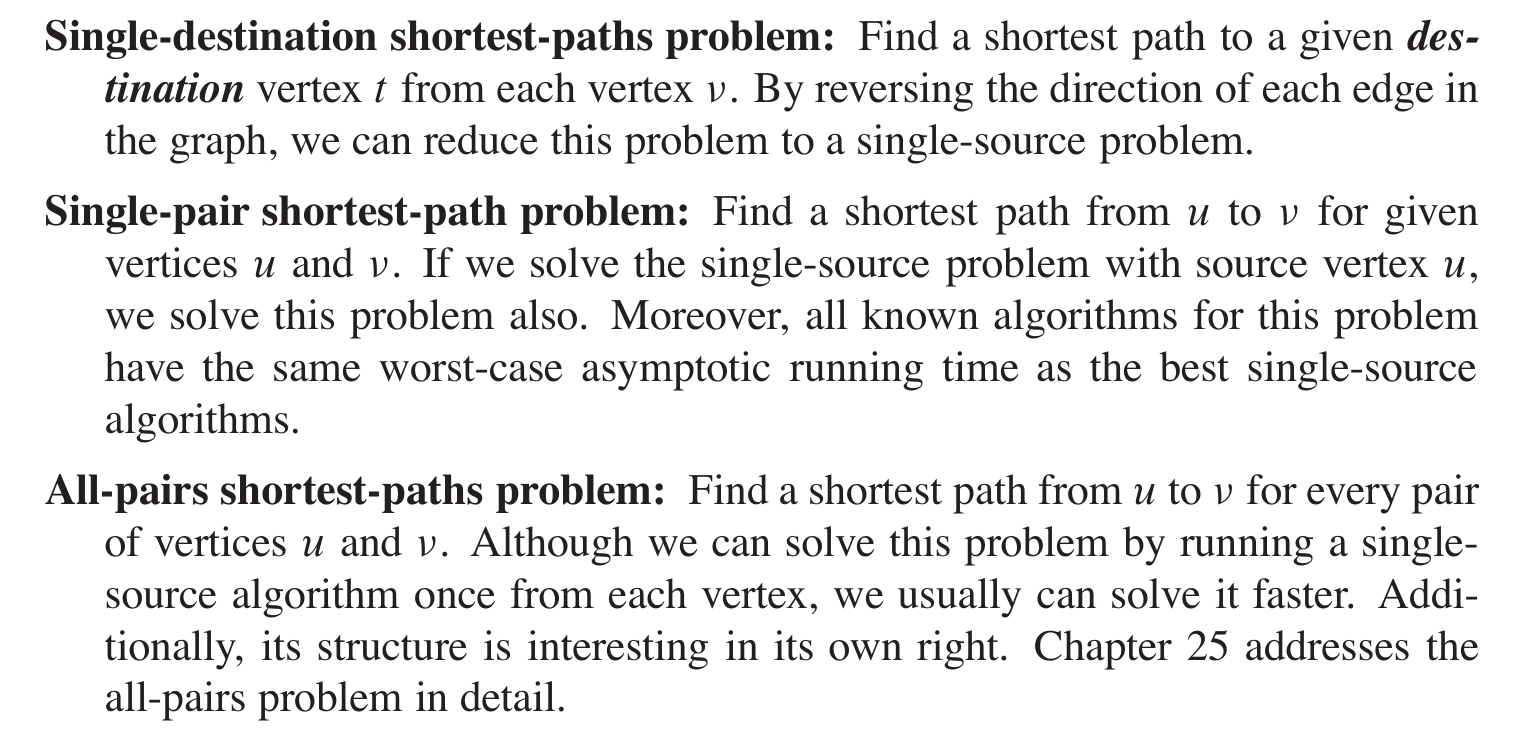
\includegraphics[scale = 0.3]{sssp1.png}
    \caption{the variants of single-source shortest paths problems}
    \label{1}
\end{figure}
其中这里的all-paired shortest paths problems 是我们在25中面对的问题. 

\subsection{optimal structure of shortest paths}
rt. 最短路径具有优化子结构, 即, 
\begin{theorem}
最短路径的{\bf 子路径}也是{\bf 最短路径}
\end{theorem}
\begin{proof}
    trivial!
\end{proof}

\subsection{representation of shortest paths} 
这涉及到前面我还没看的部分, 即无向无权图的最短路径求解. 这里我们涉及 \textbf{predecessor} , 符号 $\pi  $ 的出现说明其和 \textbf{predecessor} 有关. 比如说: 
$v. \pi$ 是 $v$ 的一个前驱
%目前并不清楚这个前驱是哪里来的. 
\begin{definition}[predecessor subgraph]
$G_{\pi} = \left(V_{\pi  } , E_{\pi}\right)$ 是 predecessor subgraph , 其中 
$$V_{\pi} = \left\{v \in V : v.\pi \ne \varnothing\right\}\cup \left\{s\right\}$$ 
s 是source, 
并且
$$E _{\pi   } = \left\{ \left(v.\pi , v\right):v \in V_{\pi} - \left\{s\right\} \right\}$$
\end{definition}

虽然这里定义并不是非常清晰, 比如说 $v.\pi$ tm的是什么我也不太清楚. 但是我们这里可以用语言将其描述清楚:
\\ [8pt]
\noindent single-source shortest paths 问题其实就是求出下面这个子图 
\\$G'  = \left(V '  , E'\right)$ \\ $V'$ 是所有能够达到的点的集合, 即 $\delta \left(s , v\right) \ne \infty$
\\并且 $G'$ 是一个树, 并且这个树上的任意一个节点 $v$ , 则 $v$ 和 $s$ 之间的距离最短. 

这就是用另一种方法说了一边我们要求什么. 
超, 我也不知道为什么要说什么 predecessor subgraph . 可能是说 $G'$ 是 $G_{\pi    }$ 的子图. 并不是很懂
\subsection{relaxation}
\subsubsection{initializing single source}
我们使用 $v.d$ 表示目前已知的 $v, s$ 之间的距离. 称为 \textbf{shortest path estimate}. 这时可以补充上面的 $v.\pi$ 了: $v.\pi$ 就是目前已知的 "最短路径上" $v$ 的前驱.

\begin{figure}[H]
    \centering
    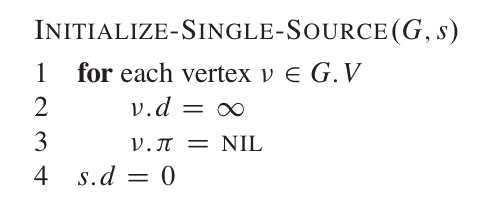
\includegraphics[scale = 0.5]{sssp2.png}
    \caption{初始化的伪代码}
    \label{iss}
\end{figure}
ss

\subsubsection{relaxation: code and definition}

relaxation是一个很简单但是很重要的操作. relaxation这个词我们之前就已经见过了, 可能有人那时候开始就觉得: 
松弛是什么叫法啊. 总之, 确实不够自然. 
应该可以将其称为renew或者update. 

\begin{definition}[relaxation]
% left empty
\end{definition}
\begin{figure}[H]
    \centering
    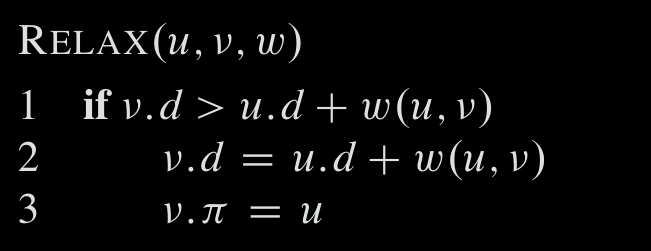
\includegraphics[scale = 0.5]{sssp3.png}
    \caption{code}
    \label{relaxation}
\end{figure}

意思即为, $u$ 到 $v$ 的一个松弛, 如果说走到 $u$ 然后走到 $v$ 的长度更短, 我们就更新 $v.d$ 目前最短路径长度; $v.\pi$ $v$ 的前驱, i.e. 更新为 $u$
而 \verb|relaxation| 只需要常数时间. 

% quotation 的间距好像也不是很理想.
% quotation 好像很难加上caption
% 说起来figure的caption的前缀很难改欸.
\begin{quotation}
Each algorithm in this chapter calls INITIALIZE-SINGLE-SOURCE and then repeatedly relaxes edges. Moreover, relaxation is the only means by which shortest
path estimates and predecessors change. The algorithms in this chapter differ in
how many times they relax each edge and the order in which they relax edges. Dijkstra's algorithm and the shortest-paths algorithm for directed acyclic graphs relax
each edge exactly once. The Bellman-Ford algorithm relaxes each edge $\left| V \right|  -1$
times.
\end{quotation}


\subsection{some property}

你可以将两点之间的最短路径视为一个度量, 即, $\delta \left(u ,v\right)$ , 至少在正权图中, 满足度量的三个性质: 

\begin{itemize}
% 你奶奶的, 怎么修改item的间距来着?
    \item 1. 正定性: $\delta \left(v, u\right) \ge 0$
    \item 2. 忘了什么性: $\delta \left(u,v\right) = 0   \implies u = v$ 
    \item 3. 三角不等式. $\delta (u, v ) + \delta \left(v , w\right) \ge \delta (u ,w)$
\end{itemize}

至少这样好像挺有意思的. 然后虽然这样说并不是很好, 但是, 书本上涉及的这部分性质, 其实是非常直观并且感觉很明显的事情. 
只有这不等式没有如此显然. 
\subsection{an outline copied from textbook}
Section 24.1 presents the Bellman-Ford algorithm, which solves the single-source
shortest-paths problem in the general case in which edges can have negative weight.
The Bellman-Ford algorithm is remarkably simple, and it has the further benefit
of detecting whether a negative-weight cycle is reachable from the source. 
Section 24.2 gives a linear-time algorithm for computing shortest paths from a single
source in a directed acyclic graph. Section 24.3 covers Dijkstra's algorithm, which
has a lower running time than the Bellman-Ford algorithm but requires the edge
weights to be nonnegative. Section 24.4 shows how we can use the Bellman-Ford
algorithm to solve a special case of linear programming. Finally, Section 24.5
proves the properties of shortest paths and relaxation stated above.

We require some conventions for doing arithmetic with infinities. We shall assume
that for any real number $a \ne \infty$, we have $a + \infty  = \infty + a = \infty$. Also, to
make our proofs hold in the presence of negative-weight cycles, we shall assume
that for any real number $a \ne 1$, we have $a + \left(- \infty\right) = \left(  - \infty\right) + a =  - \infty$

All algorithms in this chapter assume that the directed graph G is stored in the
adjacency-list representation. Additionally, stored with each edge is its weight, so
that as we traverse each adjacency list, we can determine the edge weights in $O \left(1\right)$ 
time per edge.
\section{Bellman-Ford algorithm}
\subsection{an introd}
\subsection{algorithm}
\subsection{negative weighted cycles}
\subsection{the prf of theorem}
\section{Dijikstra algorithm}
\subsection{an review}
\subsection{algorithm}
\subsection{the prf of algorithm}
\end{document}